\begin{frame}
\frametitle{Civil Aviation in Australia}
\begin{itemize}
\item<1-> Federally regulated by Civil Aviation Safety Authority (CASA).
\item<2-> Services, such as weather, provided by Airservices Australia.
\end{itemize}
\end{frame}

\begin{frame}
\frametitle{Civil Aviation in Australia}
\begin{block}{and we don't want this to happen}
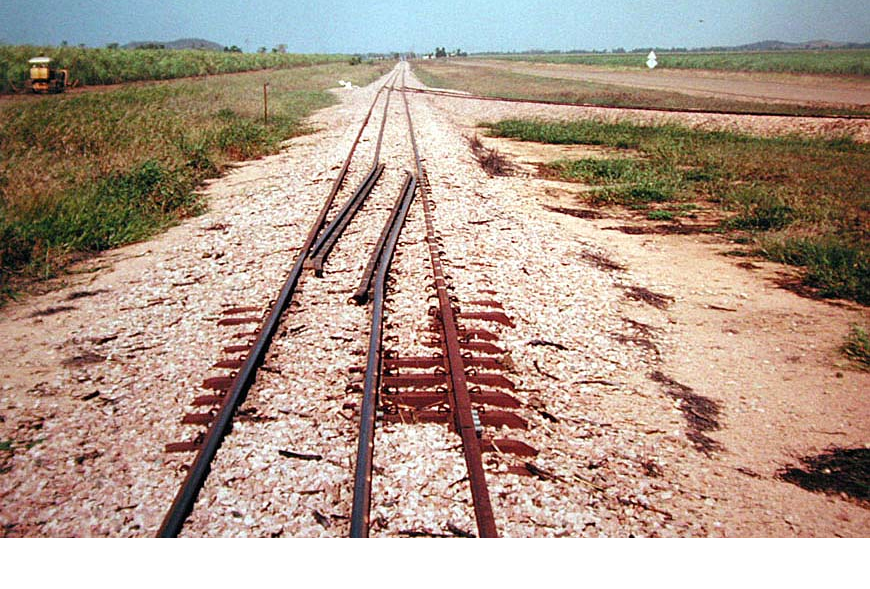
\includegraphics[height=0.5\textheight,natwidth=870,natheight=589]{image/railway-gauge.png}
\end{block}
\end{frame}

\begin{frame}
\frametitle{Civil Aviation in Australia}
\begin{block}{so these also exist}
\begin{itemize}
\item<1-> International Air Services Commission, Australia (IASC).
\item<2-> International Civil Aviation Organisation (ICAO).
\end{itemize}
\end{block}
\end{frame}

\begin{frame}
\frametitle{Civil Aviation in Australia}
\begin{block}{Australian aviation legislation}
\begin{itemize}
\item<1-> Australian Commonwealth, Civil Aviation Act 1988.
\item<2-> Under CAA1988, is Civil Aviation Safety Regulations 1998.
\item<3-> The Civil Aviation Regulation 1988 (CAR) is replaced by CASR.
\end{itemize}
\end{block}
\end{frame}

\begin{frame}
\frametitle{Civil Aviation in Australia}
\begin{block}{CASR 61.345 \emph{(pilot logbooks)}}
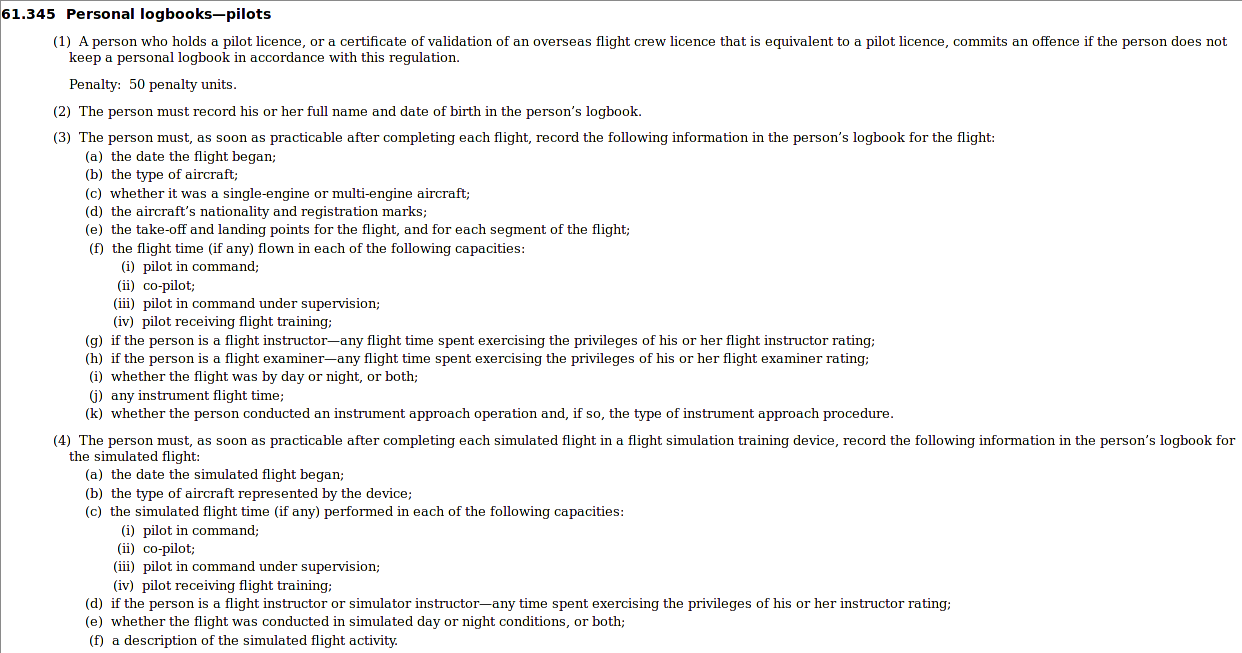
\includegraphics[height=0.6\textheight,natwidth=870,natheight=589]{image/casr-logbook.png}
\end{block}
\end{frame}

\begin{frame}
\frametitle{Civil Aviation in Australia}
\begin{block}{CASR 61.345 \emph{(pilot logbooks)}}
Are electronic logbooks OK?
\end{block}
\end{frame}

\begin{frame}
\frametitle{Civil Aviation in Australia}
\begin{block}{Yes. CASR 61.365(3)}
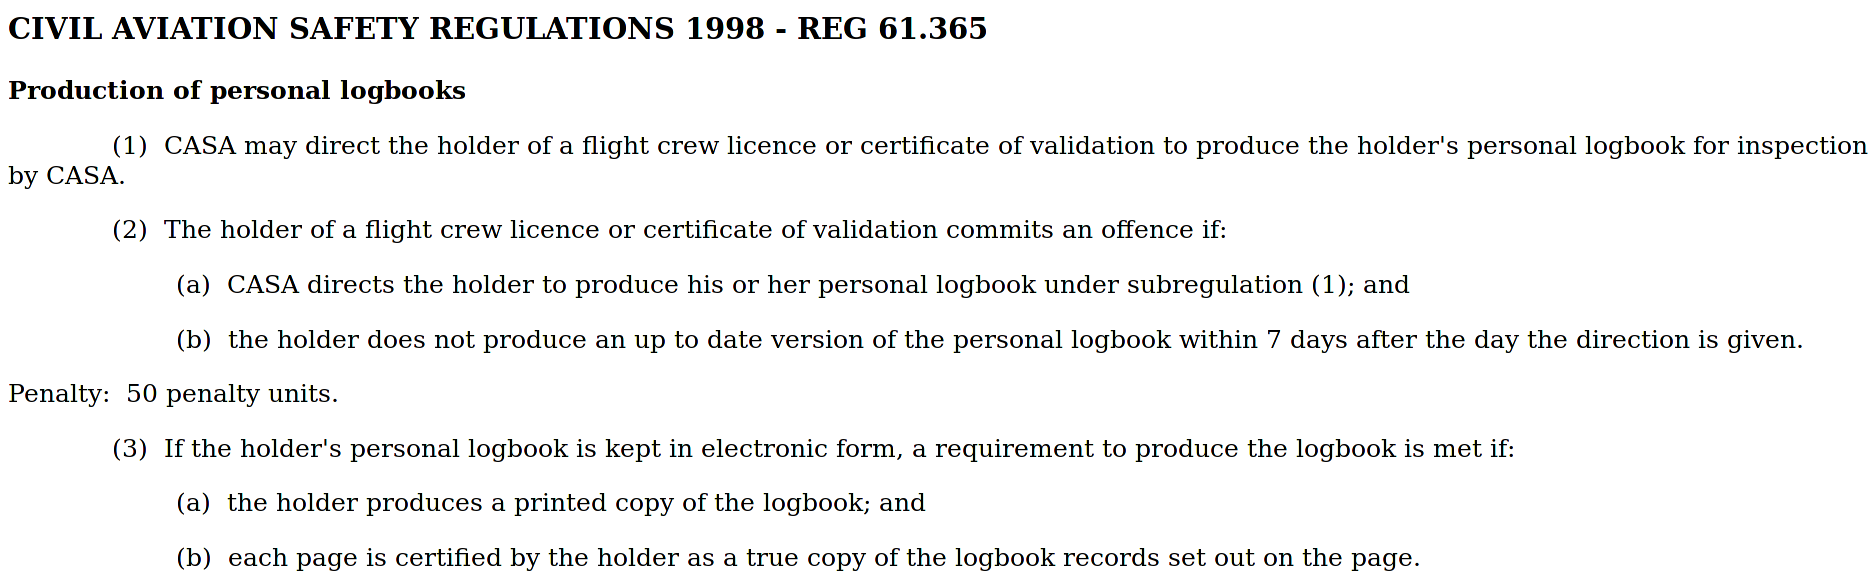
\includegraphics[height=0.3\textheight,natwidth=1871,natheight=575]{image/casr-logbook-production.png}
\end{block}
\end{frame}

\begin{frame}
\frametitle{Pilot logbooks}
\begin{block}{Introducing the pilot logbook cottage industry}
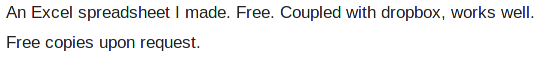
\includegraphics[height=0.1\textheight,natwidth=541,natheight=59]{image/logbook-1.png}
\end{block}
\end{frame}

\begin{frame}
\frametitle{Pilot logbooks}
\begin{block}{Introducing the pilot logbook cottage industry}
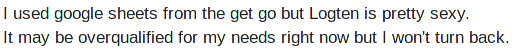
\includegraphics[height=0.1\textheight,natwidth=518,natheight=50]{image/logbook-2.png}
\end{block}
\end{frame}

\begin{frame}
\frametitle{Pilot logbooks}
\begin{block}{Introducing the pilot logbook cottage industry}
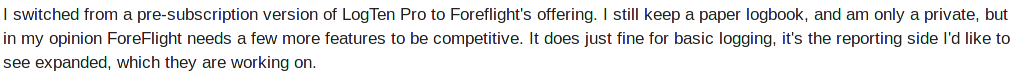
\includegraphics[height=0.08\textheight,natwidth=1024,natheight=76]{image/logbook-3.png}
\end{block}
\end{frame}

\begin{frame}
\frametitle{Pilot logbooks}
\begin{block}{Introducing the pilot logbook cottage industry}
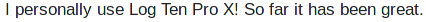
\includegraphics[height=0.05\textheight,natwidth=426,natheight=22]{image/logbook-4.png}
\end{block}
\end{frame}

\begin{frame}
\frametitle{Pilot logbooks}
\begin{block}{Introducing the pilot logbook cottage industry}
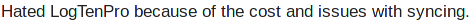
\includegraphics[height=0.05\textheight,natwidth=471,natheight=23]{image/logbook-5.png}
\end{block}
\end{frame}

\begin{frame}
\frametitle{Pilot logbooks}
\begin{block}{Introducing the pilot logbook cottage industry}
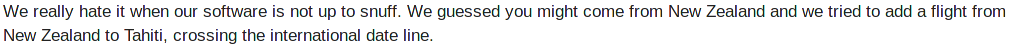
\includegraphics[height=0.05\textheight,natwidth=1015,natheight=49]{image/logbook-6.png}
\end{block}
\end{frame}

\begin{frame}
\frametitle{Pilot logbooks}
\begin{block}{Introducing the pilot logbook cottage industry}
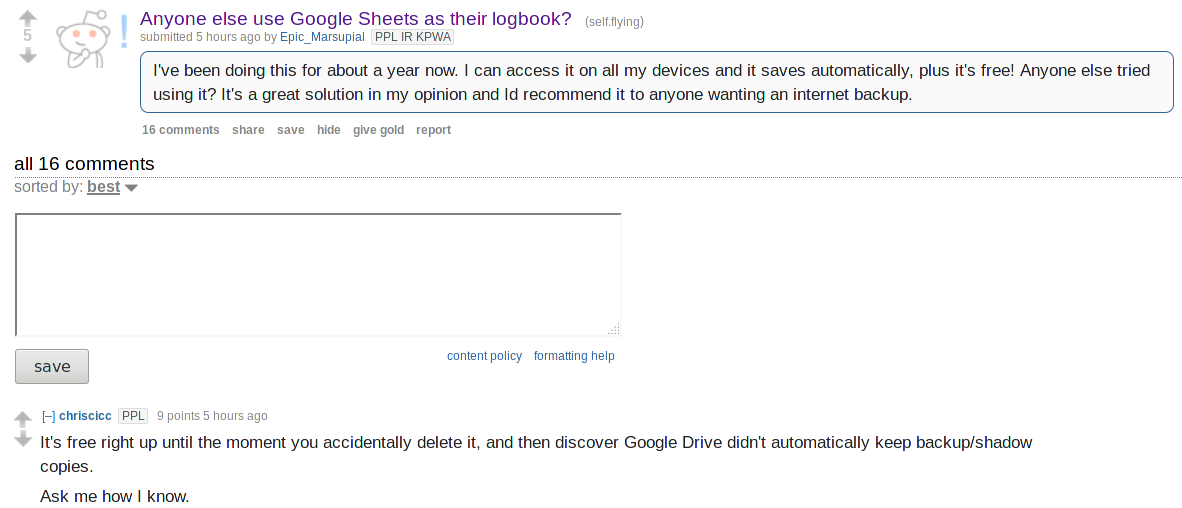
\includegraphics[height=0.4\textheight,natwidth=1182,natheight=508]{image/logbook-7.png}
\end{block}
\par
\tiny{\emph{01 August 2016}}
\end{frame}

\begin{frame}
\frametitle{Pilot logbooks}
\begin{block}{This is me, \textbf{when not flying}}

\includegraphics[height=0.5\textheight,natwidth=750,natheight=600]{image/holy-shit.png}
\end{block}
\end{frame}

\begin{frame}
\frametitle{Pilot logbooks \emph{for responsible pilots}}
\begin{block}{Pilot logbook requirements}
\begin{itemize}
\item<1-> Data loss impossible, including logbook history, with merge.
\item<2-> First-class logbook-related values for composition.
\item<3-> Values that can \emph{close over} other values.
\item<4-> Ability for \emph{arbitrary} reporting.
\item<5-> \textbf{You can see where I am going, innit?}
\end{itemize}
\end{block}
\end{frame}

\begin{frame}
\frametitle{Pilot logbook}
\begin{block}{A responsible, CASR 61.x compliant pilot uses}
\begin{itemize}
\item<1-> Haskell data type (sums and products) for logbook.
\item<1-> Lenses for querying and reporting.
\item<1-> Pilot logbook zipper for navigating a logbook.
\item<1-> A pretty-printer to meet CASR 61.365 requirements.
\item<1-> Revision control (git) for maintaining zero data loss.
\item<1-> Publishes open-source logbook libraries.
\end{itemize}
\end{block}
\end{frame}

\begin{frame}[fragile]
\frametitle{Use-case}
\begin{block}{Query: Aviation Reference Number (ARN) of logbook owner}
\begin{lstlisting}[style=haskell,basicstyle=\scriptsize\ttfamily,mathescape]
digitlist :: Prism$'$ Int [Digit]
arn :: Lens$'$ Aviator [Digit]
logbookaviator :: Lens$'$ (Logbook a b c d) Aviator
mylogbook :: Logbook a b c d

$\lambda$> mylogbook ^.
      logbook . logbookaviator . arn . re digitlist
1007036
\end{lstlisting}
\end{block}
\end{frame}

\begin{frame}[fragile]
\frametitle{Use-case}
\begin{block}{Modify: Set the digit at index 2 of the ARN to 5}
\begin{lstlisting}[style=haskell,basicstyle=\scriptsize\ttfamily,mathescape]
arn :: Lens$'$ Aviator [Digit]
logbookaviator :: Lens$'$ (Logbook a b c d) Aviator

$\lambda$> :t logbook . logbookaviator . arn %~
      \d -> d & ix 2 .~ x5
Logbook a b c d -> Logbook a b c d
\end{lstlisting}
\end{block}
\end{frame}

\begin{frame}[fragile]
\frametitle{Use-case}
\begin{block}{Modify: Upper-case the surname of the logbook owner}
\begin{lstlisting}[style=haskell,basicstyle=\scriptsize\ttfamily,mathescape]
logbookaviator :: Lens$'$ (Logbook a b c d) Aviator
surname :: Lens$'$ Aviator String
map toUpper :: String -> String

$\lambda$> :t over
      (logbook . logbookaviator . surname)
      (map toUpper)
Logbook a b c d -> Logbook a b c d
\end{lstlisting}
\end{block}
\end{frame}

\begin{frame}[fragile]
\frametitle{Use-case}
\begin{block}{Query: Aircraft from all flights}
\begin{lstlisting}[style=haskell,basicstyle=\scriptsize\ttfamily,mathescape]
logbookentries :: Lens (Logbook a b c d) (Entries a b c d)
_Wrapped :: Iso$'$ (Entries a b c d) [Entry a b c d]
folded :: Foldable f => IndexedFold Int (f a) a 
_AircraftFlightEntry ::
      Prism$'$ (Entry a b c d) (AircraftFlight, a)
flightaircraft :: Lens$'$ AircraftFlight Aircraft
mylogbook :: Logbook a b c d

$\lambda$> :t mylogbook ^..
      logbook .
      logbookentries .
      _Wrapped .
      folded .
      _AircraftFlightEntry . _1 .
      flightaircraft
[Aircraft]
\end{lstlisting}
\end{block}
\end{frame}

\begin{frame}[fragile]
\frametitle{Use-case}
\begin{block}{Query: Find first flight in aircraft registration VH-VVO}
\begin{lstlisting}[style=haskell,basicstyle=\scriptsize\ttfamily,mathescape]
logbookentries :: Lens (Logbook a b c d) (Entries a b c d)
_AircraftFlightEntry ::
      Prism$'$ (Entry a b c d) (AircraftFlight, a)
flightaircraft :: Lens$'$ AircraftFlight Aircraft
aircraftRegistration :: Lens$'$ Aircraft String

$\lambda$> :t findOf
      ( logbook . 
        logbookentries . 
        _Wrapped . 
        folded . 
        _AircraftFlightEntry . _1)
        ( elemOf
          (
            flightaircraft . 
            aircraftRegistration)
          "VH-VVO")
      mylogbook
Maybe AircraftFlight
\end{lstlisting}
\end{block}
\end{frame}

\begin{frame}[fragile]
\frametitle{Use-case}
\begin{block}{Print: pretty-print all exam results}
\begin{lstlisting}[style=haskell,basicstyle=\scriptsize\ttfamily,mathescape]
_ExamEntry ::
      Prism$'$ (Entry a b c d) (Exam, c)
examResult :: Lens$'$ Exam Int
examResultMaximum :: Lens$'$ Exam Int

$\lambda$> mapMOf_
      ( logbook . logbookentries .
        _Wrapped . folded .
        _ExamEntry . _1 .
        runGetter
          ((\x y -> show x ++ $\text{" out of "}$ ++ show y) <$\text{\$}$>
          Getter examResult <*>
          Getter examResultMaximum)
        )
      putStrLn
      mylogbook
31 out of 40
38 out of 40
38 out of 40
\end{lstlisting}
\end{block}
\end{frame}

\begin{frame}[fragile]
\frametitle{Use-case}
\begin{block}{Query: All aircraft flights as pilot in-command}
\begin{lstlisting}[style=haskell,basicstyle=\scriptsize\ttfamily,mathescape]
logbookentries :: Lens (Logbook a b c d) (Entries a b c d)
_AircraftFlightEntry ::
      Prism$'$ (Entry a b c d) (AircraftFlight, a)
flightaircraft :: Lens$'$ AircraftFlight Aircraft
aircraftRegistration :: Lens$'$ Aircraft String

$\lambda$> :t
      mylogbook ^..
      logbook .
      logbookentries .
      _Wrapped .
      folded .
      _AircraftFlightEntry . _1 .
      filtered
        (elemOf (command . _InCommand) ())
[AircraftFlight]
\end{lstlisting}
\end{block}
\end{frame}

\begin{frame}[fragile]
\frametitle{Use-case}
\begin{block}{Query: Total day hours as pilot in-command}
\begin{lstlisting}[style=haskell,basicstyle=\scriptsize\ttfamily,mathescape]
$\lambda$> foldOf
      ( logbook .
        logbookentries .
        _Wrapped .
        folded .
        _AircraftFlightEntry . _1 .
        filtered
          (elemOf (command . _InCommand) ()) .
        daynight .
        dayDayNight
      )
      mylogbook
TimeAmount {_hours = 4, _tenthofhour = 8}
\end{lstlisting}
\end{block}
\end{frame}

\begin{frame}[fragile]
\frametitle{Use-case}
\begin{block}{Print the entire logbook to a single, printable HTML web page}
\begin{lstlisting}[style=haskell,mathescape]
$\lambda$> :t htmlLogbook mylogbook
Html ()
\end{lstlisting}
\end{block}
\href{http://logbook.aviation.tmorris.net/}{http://logbook.aviation.tmorris.net/}
\end{frame}

\begin{frame}[fragile]
\frametitle{Use-case}
\begin{block}{Query of arbitrary obtuseness}
All flights where, if the departure and arrival date is the same day (UTC), and that date-of-month is a multiple of 7, unless either there was an intermediate flight path point of YSCN, or the time the logbook owner was PiC for the first three legs of the flight, is between 2.0 hours and the total sum of hours of dual flight in aircraft registered VH-AFR.

\emph{code too big to fit on screen}
\end{block}
\end{frame}

